\documentclass[11pt,french,french]{article}
\usepackage{lmodern}
\usepackage{amssymb,amsmath}
\usepackage{ifxetex,ifluatex}
\usepackage{fixltx2e} % provides \textsubscript
\ifnum 0\ifxetex 1\fi\ifluatex 1\fi=0 % if pdftex
  \usepackage[T1]{fontenc}
  \usepackage[utf8]{inputenc}
\else % if luatex or xelatex
  \ifxetex
    \usepackage{mathspec}
    \usepackage{xltxtra,xunicode}
  \else
    \usepackage{fontspec}
  \fi
  \defaultfontfeatures{Mapping=tex-text,Scale=MatchLowercase}
  \newcommand{\euro}{€}
\fi
% use upquote if available, for straight quotes in verbatim environments
\IfFileExists{upquote.sty}{\usepackage{upquote}}{}
% use microtype if available
\IfFileExists{microtype.sty}{%
\usepackage{microtype}
\UseMicrotypeSet[protrusion]{basicmath} % disable protrusion for tt fonts
}{}
\usepackage[margin=1in]{geometry}
\ifxetex
  \usepackage{polyglossia}
  \setmainlanguage{}
\else
  \usepackage[shorthands=off,french]{babel}
\fi
\usepackage{graphicx}
\makeatletter
\def\maxwidth{\ifdim\Gin@nat@width>\linewidth\linewidth\else\Gin@nat@width\fi}
\def\maxheight{\ifdim\Gin@nat@height>\textheight\textheight\else\Gin@nat@height\fi}
\makeatother
% Scale images if necessary, so that they will not overflow the page
% margins by default, and it is still possible to overwrite the defaults
% using explicit options in \includegraphics[width, height, ...]{}
\setkeys{Gin}{width=\maxwidth,height=\maxheight,keepaspectratio}
\ifxetex
  \usepackage[setpagesize=false, % page size defined by xetex
              unicode=false, % unicode breaks when used with xetex
              xetex]{hyperref}
\else
  \usepackage[unicode=true]{hyperref}
\fi
\hypersetup{breaklinks=true,
            bookmarks=true,
            pdfauthor={},
            pdftitle={},
            colorlinks=true,
            citecolor=blue,
            urlcolor=blue,
            linkcolor=magenta,
            pdfborder={0 0 0}}
\urlstyle{same}  % don't use monospace font for urls
\setlength{\parindent}{0pt}
\setlength{\parskip}{6pt plus 2pt minus 1pt}
\setlength{\emergencystretch}{3em}  % prevent overfull lines
\setcounter{secnumdepth}{5}

%%% Use protect on footnotes to avoid problems with footnotes in titles
\let\rmarkdownfootnote\footnote%
\def\footnote{\protect\rmarkdownfootnote}


  \title{Analyse statistique et empirique des modèles\\
de Word Embedding sur Twitter}
    \author{Kim Antunez, Romain Lesauvage, Alain
Quartier-la-Tente\\[2\baselineskip]sous l'encadrement de Benjamin Muller
(Inria)}
    \date{}
  

\begin{document}

\maketitle


\section{Contexte}\label{contexte}

Grâce à l'évolution des méthodes d'apprentissage profond (\emph{Deep
Learning}), l'appréhension du langage naturel est aujourd'hui devenu une
discipline à part entière (\emph{Natural Language Processing}). Ce
succès s'explique en partie grâce à l'émergence de techniques non
supervisée d'apprentissage de représentation de structures
linguistiques. Les méthodes de \emph{word embedding} (« plongement
lexical » en français) permettent de représenter chaque mot d'un
dictionnaire par un vecteur de nombres réels afin que les mots qui
apparaissant dans des contextes similaires possèdent des vecteurs
correspondants qui sont relativement proches. Les modèles
\textbf{word2vec}, développés par une équipe de recherche chez Google
sous la direction de Tomas Mikolov, sont parmi les plus célèbres et sont
ceux sur lesquels se concentreront notre projet.

\section{Objectif du projet}\label{objectif-du-projet}

Dans ce projet de statistiques appliquées, nous étudierons dans un
premier temps en détail et implémenterons le modèle \emph{word2vec} avec
l'architecture Skip-Gram. Danns un second temps, l'objectif est de
mettre en application ce modèle sur une base de données créée à partir
de plusieurs millions de tweets écrits en France sur la période
2013-2017 et de mettre en oeuvre à partir de cela des techniques
d'analyse de sentiments, afin d'arriver à comparer nos résultats avec
certains indicateurs de l'Insee par exemple sur l'opinion des ménages.

\section{Travail effectué}\label{travail-effectuuxe9}

\subsection{Compréhension du
modèle}\label{compruxe9hension-du-moduxe8le}

Nous avons débuté le projet en nous imprégnant du champ des méthodes de
NLP et même de Deep-learning qui nous était jusqu'alors inconnu. Pour
cela nous avons lu les articles présentés dans la bibliographies ainsi
que d'autres articles de blogs, en particulier concernant
l'implémentation sur python de ces modèles. Nous avons consacré une
grande partie de notre temps dans la compréhension du modèle.

Le modèle \emph{word2vec} consiste à représenter les mots d'un corpus
sous forme d'un vecteurs de nombres réels. Pour cela, le principe est
d'entraîner un réseau de neurones sur une tâche factive, consistant à
prévoir le lien entre des mots \emph{focus} et leur contexte, et de
récupérer les poids issus de cet entraînement. Ce sont ces poids qui
seront utilisés comme représentation vectorielle des mots.

Il y a deux architectures possibles pour ce modèle :

\begin{itemize}
\item  \textit{Continuous bags of words} où l'idée est de prédire à partir des mots du contexte le mot focus sur lequel on se trouve ;
\item \textit{Skip-gram}, où l'idée est de partir d'un mot focus est de prédire, pour chaque mot, la probabilité d'être dans le contexte de ce mot focus.
\end{itemize}

C'est cette dernière approche que nous avons privilégié dans notre
projet. Nous avons donc passé du temps à comprendre le fonctionnement du
modèle avec cette architecture afin de l'implémenter.

Nous pouvons résumer l'algorithme en quelques étapes :

\begin{itemize}
\item Nous partons d'une matrice de poids en entrée et en sortie, dont la taille sera fixée par le nombre de mots de notre vocabulaire et la dimension des vecteurs que nous désirons en sortie. 
\item L'agorithme parcourt ensuite chaque phrase du corpus de texte, en sélectionnant aléatoirement un couple formé d'un mot focus et d'un mot contexte (le contexte étant défini avec une certaine taille de fenêtre) sur lequel seront appliqués les opérations permettant la mise à jour de la matrice des poids.
\item L'opération est répétée un certain nombre de fois fixé au préalable.
\end{itemize}

En sortie, on a ainsi à disposition deux matrices de poids utilisée pour
former nos vecteurs. Empiriquement, il est souvent fait la moyenne de
ces deux matrices c'est donc ce que l'on a décidé de faire également.

\subsection{Implémentation du
modèle}\label{impluxe9mentation-du-moduxe8le}

Toute la première partie de notre travail a principalement consisté en
l'implémentation du modèle, une fois que nous avons compris celui-ci.
Afin de nous approprier au maximum ces nouvelles méthodes, nous avons
décidé d'implémenter tous les trois individuellement le modèle sur
Python en utilisant la librairie Pytorch avant de mettre en commun nos
codes. De cette manière, nous avons pu chacun approfondir les points qui
nous semblaient les plus flous et arriver à une mouture de modèle qui
compile.

L'implémentation du modèle s'est déroulée en deux étapes. En effet, nous
avons commencé par implémenter une version plus simple du
\emph{word2vec} en utilisant une fonction \emph{softmax}. Cela induit de
calculer à chaque fois des informations sur tous les mots de notre
corpus et donc, algorithmiquement, cette solution n'est pas viable sur
les corpus trops gros, mais cela nous a permis de prendre en main à la
fois les données et les étapes importantes du modèle. Nous avons réussi
à aboutir à quelque chose qui donnait des résultats concluants donc nous
sommes passés à une version plus élaborée du modèle et plus optimisée.
L'idée est de voir qu'il n'est pas nécessaire de mettre à jour à chaque
étape de l'algorithme toutes les lignes des matrices de poids mais que
l'on peut seulement s'intéresser au mot contexte sur lequel on travail.
Cependant, puisqu'en faisant ça on sur-estime l'effet de ce mot, l'idée
est de s'intéresser à des mots qui ne sont pas dans le contexte, qu'on
appelle \emph{negative sampling} pour lesquels on va chercher à
minimiser l'impact. En partant de la version simplifiée du modèle que
nous avons réussi à mettre en oeuvre et une fois que nous avons compris
comment il fallait prendre en compte ces \emph{negative samplings} dans
notre fonction de coût, nous avons réussi à implémenter une version
quasi-définitive du modèle qui est conforme au papier de Mikolov.

\subsection{Evaluation du modèle
implémenté}\label{evaluation-du-moduxe8le-impluxe9mentuxe9}

Malgré leurs utilisations presque généralisées, très peu de travaux
théoriques expliquent ce qui est réellement capturé par ces
représentations de mots. C'est pourquoi l'évaluation de l'efficacité de
ce modèle ne peut se faire qu'à l'aide de méthodes empiriques. Nous
avons donc réfléchi, conjointement avec notre tuteur, aux différentes
manières qui s'offraient à nous pour mesurer l'efficacité de notre
modèle ainsi implémenté. Avant de s'attaquer à notre jeu de données
complet, nous avons décidé d'effectuer une évaluation sur des données
fictives.

L'idée est de se dire que si l'on crée un corpus fictif, basé sur dix
couples, pour lesquel on maîtrise entièrement le contexte, alors, en
construisant des phrases à partir de cela et de mots bruits, nous
devrions avoir en sortie des résultats concluants. Nous avons donc créé
un corpus à partir de ces règles : nous nous sommes fixés dix couples,
pour lequels on a associé dix mots contextes différents et nous avons
formé 10 000 phrases de test en tirant aléatoirement, pour chaque
phrase, un mot d'un couple, cinq mots du contexte et trois mots bruits.
En mélangeant les mots tirés, nous avons ainsi obtenu un corpus fictif
sur lequel nous avons pu travailler.

Nous avons retenu principalement trois méthodes d'évaluations pour
étudier les vecteurs obtenus en sortie du modèle :

\begin{itemize}
 \item La \textit{similarité cosinus}, qui consiste à calculer le cosinus de l'angle entre deux vecteurs de dimension $n$ et d'utiliser cette mesure comme similarité, ainsi un cosinus de 1 indiquera deux vecteurs identiques, -1 deux vecteurs opposés et 0 deux vecteurs indépendants.
 \item L'\textit{ACP} qui consiste à projeter nos vecteurs sur des axes, appelés composantes principales, en maximisant la variance résiduelle du projeté. 
 \item L'algorithme \textit{T-SNE}, ou \textit{t-distributed Stochastic Neighbor Embedding}, qui permis de compléter et même d'améliorer l'ACP pour les grandes dimensions. Il s'agit d'un algorithme stochastique qui permet l'apparition de clusters de points proches.
\end{itemize}

\begin{figure}
\centering
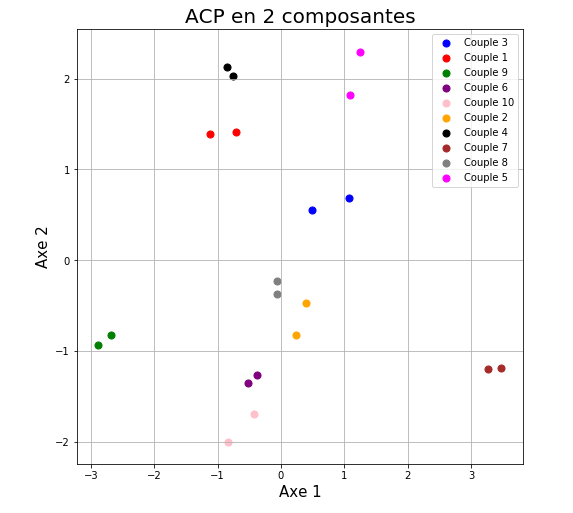
\includegraphics[width=0.50000\textwidth]{acp_fictif.png}
\caption{ACP réalisée sur le corpus de données fictives}
\end{figure}

Nous avons donc mis en oeuvre ces trois techniques sur notre corpus
fictif et les résultats ont été très concluants. Nous avons bien vu
grâce à la similarité cosinus que les vecteurs de nos couples étaient
très proches. L'ACP et l'algorithme t-SNE ont aussi permis de repérer
les couples et les mots contextes différents (Figure 1).

\section{Perspectives}\label{perspectives}

\subsection{Implémentation et
évaluation}\label{impluxe9mentation-et-uxe9valuation}

Maintenant que nous avons évalué notre modèle sur les données fictives,
il nous reste encore quelques étapes à réaliser afin d'avoir un modèle
``propre''.

Tout d'abord, nous devons finir la mise en commun de nos trois codes
afin de ne garder qu'une seule version du modèle que nous devrons
ensuite faire tourner sur les données réelles qui sont à notre
disposition. Nous allons procéder par étapes, d'abord en faisant tourner
le modèle sur 100 000 tweets, puis 1 000 000, puis sur l'ensemble de la
base. Une fois que le modèle aura tourné sur l'ensemble des tweets, nous
pourrons récupérer nos vecteurs mais nous devrons aussi procéder à
l'évaluation du modèle.

En plus de mettre en oeuvre les mêmes techniques que sur le corpus
fictif, nous pensons également nous baser sur des résultats issus du
\emph{Human Judgment Agreement}. Il s'agit d'une expérience qui a été
réalisées auprès de volontaires et qui a permis de mesurer une
similarité entre des couples de mots du point de vue humain. L'idée
serait alors de comparer les résultats obtenus par cette expériences et
les réulstats obtenus par notre modèle.

\subsection{Analyse}\label{analyse}

Tout le travail d'analyse à partir de la base de données exhaustive des
tweets reste à effectuer. Une fois que nous aurons nos vecteurs qui
représenteront les mots du corpus, l'idée est de pouvoir les utiliser
afin d'en tirer quelque chose. Puisque notre groupe est formé de trois
administrateurs de l'Insee, nous avons décidé en accord avec notre
tuteur d'essayer d'orienter l'analyse vers la statistique publique. Nous
avons donc contacté différentes personnes à l'Insee afin de réfléchir à
des applications directes de notre travail. L'Insee a déjà publié il y a
quelques temps un article qui permet de prévoir le PIB à partir
d'articles du Monde grâce à des méthodes de NLP. Bien sûr, notre base de
données étant différente, il ne sera pas possible de réaliser exactement
la même étude. Cependant, nous avons en tête différentes pistes :

\begin{itemize}
\item Nous pouvons regarder si si l’analyse des tweets permet de retrouver des résultats proches de ceux réalisées par les enquêtes Insee (Camme, l’enquête de conjoncture auprès des ménages) ou de toute autre enquête de la statistique publique (comme le Baromètre d’opinion de la DREES) et d’essayer de comprendre les différences. 
\item Nous pouvons également faire des tests autour des questions de sondages électoraux/participations électorales à l’approche des municipales.
\item Nous pouvons enfin nous intéresser au taux de chômage et essayer de le prévoir avec les tweets.
\end{itemize}

A priori, notre idée est plutôt de rester sur la comparaison avec des
enquêtes comme l'enquêtes Camme de l'Insee, mais nous gardons bien en
tête les limites liées au fait même d'utiliser des tweets et sur la
profondeur temporelle de nos données. En effet, beaucoup d'enquêtes sont
trimestrielles et nous ne pourrions alors qu'avoir qu'un faible nombre
de points à notre disposition.

\end{document}